\documentclass[11pt,
a4paper,
oneside,
abstract=true,
bibliography=notoc,
numbers=noenddot,
toc=nolistof
]{scrreprt}
\usepackage[utf8]{inputenc}
\usepackage[OT1]{fontenc}
\usepackage[default,light,bold]{sourceserifpro}
\usepackage[light,bold]{sourcesanspro}
\usepackage[regular,bold,scale=0.9]{sourcecodepro}
\usepackage[american]{babel}
\usepackage[babel=true]{microtype}
\usepackage{amsmath,amssymb,amsfonts,amsthm,mathrsfs}
\usepackage{graphicx}
\usepackage[nospace]{varioref}
\usepackage{caption}
\usepackage{array}
\usepackage{booktabs}
\usepackage{enumitem}
\usepackage[autostyle=true]{csquotes}
\usepackage{tikz}
\usepackage{minted}
%\usepackage[backend=biber,bibstyle=ieee,citestyle=numeric-comp]{biblatex}
\setminted{fontsize=\small}
\setminted{autogobble}
\setminted{linenos}

%% Paragraph control
\clubpenalty=10000% excludes orphans
\widowpenalty=10000% excludes orphans
\displaywidowpenalty=10000% excludes widows
\setlength{\parindent}{0em} % indent on first line of a paragraph
\setlength{\parskip}{1em} % vertical distance to preceding paragraph
\linespread{1.0} % note the strange values: single spacing: 1.0, 1.5 spacing: 1.3, double spacing: 1.6

\usepackage{fancyvrb}

% Make document internal hyperlinks wherever possible. (TOC, references)
% We load this package last just to be safe. Otherwise it becomes a diva.
\usepackage[breaklinks,linkcolor=black,colorlinks=true,citecolor=black,filecolor=black]{hyperref}
\expandafter\def\expandafter\UrlBreaks\expandafter{\UrlBreaks%  save the current one
   \do\a\do\b\do\c\do\d\do\e\do\f\do\g\do\h\do\i\do\j%
   \do\k\do\l\do\m\do\n\do\o\do\p\do\q\do\r\do\s\do\t%
   \do\u\do\v\do\w\do\x\do\y\do\z\do\A\do\B\do\C\do\D%
   \do\E\do\F\do\G\do\H\do\I\do\J\do\K\do\L\do\M\do\N%
   \do\O\do\P\do\Q\do\R\do\S\do\T\do\U\do\V\do\W\do\X%
   \do\Y\do\Z\do\0\do\1\do\2\do\3\do\4\do\5\do\6\do\7\do\8\do\9}
   
% Syntax containing underlines and other symbols that LaTeX thinks to be math symbols need to be in a verbatim environment
\newcommand{\sytx}[1]{\mintinline{text}{#1}} 

\title{Flake OS\\\hspace{1em} \large AOS Final Report Group 7}
\author{Altin Alickaj \and Thierry Backes \and Florian Bütler \and Manuel Hässig}

\begin{document}

\maketitle

\tableofcontents

\chapter{Introduction}
We present our project report for the operating system we have been building for the last couple of months. 
In the final submission, we present a system describing our approaches to the milestones M0-M6 as well as the 
following individual milestones: A file system, networking, a name server and a shell.

Together, these milestones build the operating system we call Flake OS. Why is it called that?
Well --- sometimes it is a little bit flaky. While the name currently can be seen as a wordplay rather than a serious name, given more time, the system could become more elegant and sophisticated - like a snowflake, perhaps?

\chapter{Simple Shell and Power Management}
For the first milestone, we want to briefly outline the problems we faced,
the solutions we found, and the approached we followed. 
While there is not much to tell, we still want to provide a short account of this introduction into the project.

Of course, note first that we use QEMU in this milestone and it's provided UART interface.
In the specification online, we found everything necessary for a successful communication with the interface.

\section{Output}
When wanting to print a character to the screen, we wait until the graphical device is
ready and then we send it to make it appear on the screen.

\section{Input}
Input works in a similar fashion. We wait until the device says there is data to
be read and then we read it into local memory.  On the first try, we made a mistake by
confusing \mintinline{c}{0x4} with \mintinline{c}{1 << 4} and hence the third bit was checked instead of the
fourth. This let the program make progress even if there was no character,
resulting in bad performance.

\section{Simple Shell}
Implementing a simple shell requires to store every character that is entered
until the return key is pressed. This is done in a char array. The char array
allows a maximal input length of 255 characters as a first choice.  Once the return key is
entered, the string (stored in the char array) is terminated and evaluated. If
it matches an implemented command, it executes it.  As \texttt{printf} uses the function
we implemented for output, we were able to use it quite simply to print whole strings to the screen. 
We provide a \texttt{hello} and \texttt{help} command that just print some text back to the user,
otherwise the input is ignored. We also implemented the functionality of \texttt{Ctrl+C}
to abort an input. Moreover, there is the functionality of a backspace implemented
as well. This is done by moving the cursor one character back, printing a space, 
i.e. an empty character and then moving the cursor back again. To make
things a bit more aesthetic, a \texttt{\$} is printed to start an input and a newline is
started when an input is evaluated.

\section{Shutdown/Reboot}
Shutdown and reboot is all about reading the specification. We decided to use the
SMC32 calling convention and a fast call. First, we had trouble understanding what
the value of the service call range was. But it turned out it is the "Owning
entity number", i.e. 4. We also had a bug that was confusing for a while, but it
turned out, we were just so focused on getting the value right that we forgot to
call the \mintinline{asm}{smc} assembly instruction, therefore the value in the register was never
evaluated. The difference of shutdown and reboot is just an offset of 1 of the
value stored in the register. The most challenging part of this task was to
understand the specification correctly and getting the assembly instructions
right.

\chapter{Memory Allocator}

\section{Physical Frame Allocator}

\subsection{Algorithm}

I first wanted to implement a buddy allocator and implemented a reference
implementation for testing purposes outside of barrelfish and then imported that
into barrelfish as my memory allocator. Unfortunately, I struggled understanding
the concept of how capabilities are split i.e. I got that I get a new capref but
it was not clear for me what happens to the rest. Do I get another new capref
with that? After some time I figured out that it the original capability is
still untouched from the point of view of the memory allocator and the only
difference is that when I try to split the same part, I get am error from the
underlying capability management system(correct name?).

Also havent I decided how to handle the noncontinous memory regions that are
handed to the memory allocator nor how to handle memory regions that are not a
power of two in size.

All this then lead me to implement a simple first fit allocator with a doubly
linked list to get things started. Later I improved the first fit allocator to a
next fit allocator with a circular buffer.

There were more obstacles to overcome: I was puzzled first how to allocate an
object on the heap .i.e as you do with malloc in normal C programs. I then
figured out that this is the purpose of the slab allocator. There I wasnt sure
what block size to choose and how much memory the slab allocator needs. So I
went over all object I wanted to allocate and choose the biggest object in terms
of bytes as the block size and just gave the slab allocator a bunch of bytes.

As I needed a list implementation for my first attempt of implementing the
memory allocator, I added my own to the source tree. Little did I know that
there is already an implementation under collections/. However, this one anyways
uses malloc so I could use it at this stage, but still useful to know for later.
I later changed my memory allocator to natively be implemented with links so I
didn't need my list implementation anymore.

In the following I am going to discuss my implementation of a next fit memory
allocator.

(maybe explain the next fit allocator?)

\subsection{Datastructure}

As mentioned above, the datastructure for my next fit allocator is a circular
buffer.  The circular buffer is implemented as a doubly linked link list and the
smallest unit is a mmnode (memory manager node).  Each mmnode represents
continous region of memory and is linked to the next node that is represent the
next closest region of memory. The memory nodes that represent the start (lowest
memory address) and the end (highest memory address) of the memory are linked
with each other.  A node can be split into two nodes to accomodate its size to
the size of the requested memory or be merged with one of its neighbours, if
they are free.  A mmnode contains its type, wheter it is free or allocated,
pointers to its adjacent neighbours, its memory base address, its size and a
capinfo. The capinfo contains the capref and its original memory base address
and size:

\begin{minted}{c}
enum nodetype { NodeType_Free, NodeType_Allocated };

struct capinfo {
    struct capref cap;
    genpaddr_t base;
    size_t size;
};

typedef struct mmnode_t {
    enum nodetype type;
    struct capinfo capinfo;
    struct mmnode_t *prev;
    struct mmnode_t *next;
    genpaddr_t base;
    gensize_t size;
} mmnode_t;
\end{minted}

The datastructure is concluded by storing a pointer to the head of the linked
list. As it is a circular buffer, it does not really have a natural head, but
this is the pointer to the current position in the circular buffer. The memory
allocator has more in it and they will be discussed at a later point.

\begin{minted}{c}
struct mm {
    struct slab_allocator slab_allocator;
    slot_alloc_t slot_alloc;
    slot_refill_t slot_refill;
    void *slot_allocator;
    enum objtype objtype;

    mmnode_t *head;
};
\end{minted}

\subsection{Add memory}

Initially, the memory allocators head is NULL as there is no memory at the
moment available. The memory allocator gets hold of new memory from the init
process that reads that information from the bootinfo. With each new memory
region added we add another node representing this region. The memory region
comes in the form of a capref to a RAM capability. By inspecting it, we can read
its memory base address and size and create a node for it. As its our first node
its next and prev pointer point to it self and the head points to it.  As more
memory regions are added, more nodes are created and inserted before our current
head. As it may be clear we mark all these nodes as free memory.

\subsection{Alloc memory}

If any other component in barrelfish wants a ram capability, it needs to ask us.
After some initial sanity checks of the request, we now need to find a memory
region that fits the request. There are multiple parameters such as size of the
memory and its alignment i.e. it has to start on a address that is a multiple of
the alignment.  To fullfill these requirements we traverse the circular buffer
until we find a node that is marked as free and its size is large enough. If the
memory that is represented by the node is not aligned as requested, we check if
the aligned version still fits in this node and continue our traversal
otherwise.  If the node is not aligned but is still big enough, we split the
node at an aligned position into two nodes with the right one being alinged.
Splitting just inserts the new node into the circular buffer by pointing the
previous node to itself and itself to the next node. Of course we need to update
the base addresses and sizes of the nodes.  As we now have a node that fulfills
all requirements we retype the capref to the correct size for both nodes and
storing it as the result.  This is also the node we are going to start our
search from for future memory allocation request (i.e. next fit).

\subsection{Free memory}

Freeing memory reverses an allocation. We identify the correct node by
inspecting the provided capref, that gives us the base address and size.  If we
did not find the node we did not hand out this memory region and ignore the free
request.  If we found the node, we destroy the capref and marke the node as
free. Further, we check both neighbours for a possible node merge. In a node
merge we check whether they represent also physical adjacent memory regions to
our memory region. This is crucial to not try and merge the "first" and "last"
node as our data structure is a ciruclar buffer but the memory is still linear.
Also the neighbours have to be marked free as well. If that all is the case we
merge them by simple pointing the previous node to the next node.

This concludes our memory allocator.

\subsection{Partially free memory}

I have also implemented to free partial memory. We know check the incoming free
request, whether its address is represented by a node and if yes and the size is
not the whole node, we split the node according to the partial free request.
Here we have 3 cases: left aligned, middle aligned and right aligned partial
free. For left and right aligned we need to split once and for the middle
aligned we need to split the node twice. The rest works as usual afterwards as
the normal free, the only difference is that we work on a new node.

\subsection{Slab memory allocator}

Our mmnodes need some memory as well store its data. But where to take it from,
when the nodes have the be created first before memory is handed out by the
memory allocator?  This is the purpose of the slab allocator. It can hand out
memory but only of a certain block size. For the slab allocator instance used in
the memory allocator its block size is the size of a mmnode. We initially give
the slab allocator some memory from the init process and if that runs out we
have to get it from the actual memory allocator that should now be bootstrapped.
The slab allocator is used in a node split to create a new node and also when we
add some memory to the memory allocator. We return a slab on a node merge. We
also need to periodically check, whether we need to refill the slab allocator
with new memory. We do this after after each memory allocation in our memory
allocator.  Why do we even need to do that?  Well, once the slab allocator has
run out of memory and only then want to allocate more memory to it we need to
ask the memory allocator for memory but this one needs a slab to allocate
memory. So you see the problem here?

\subsection{Slot memory allocator}

To store the capref we hand out for every memory allocations we need some memory
as well. Initially it also gets some memory from the init process.  We allocate
a slot for each capref we return for an allocation request and free the slot on
a free request (at the moment, however, the slot allocator does no bookkeeping
for allocated slots).  This one also needs to be refilled and we check that
before each slot allocation. This one is even more tricky, if we run out of
slots. A slot refill needs to allocate memory, that needs a slab for its
bookkeeping that may trigger a slab refill and that requires a slot too.  For
this purpose, I also added a function that reports the number of free slots.

\section{Frame mapping}

\subsection{Page table}

Next, we need to be able to map a virtual address to a frame capability that was
derived from a ram capability that represents a pyhsical memory region.  For
this prupose we need to create a page table that is able to do this mapping.  We
have a 4 level deep page table. The first level (L0) is at a well known location
and exists already. So we only need to create the other levels on the fly as we
need them i.e. need to store a value in one of its entries.  Once we reached the
last level, we store the frame capref and are done.  The datastructure here is a
tree. Each page table stores pointers to their children.  The memory to store
the datastructure is once again done by a slab allocator (not the same one) with
some memory provided by the init process.

\subsection{Slab allocator refills}

Now, we are able to actually refill the slab allocator.  Here we first allocate
a frame capref (derived from a ram capref) and map the frame into the page table
for the given virtual address. We can then tell the slab allocator that there is
some more memory at the virtual address for its use.

\section{Tests}

To test all the above discussed functionalities I wrote some tests. They include
alternating memory allocations and frees of one base page i.e. 4KB (the
iterations may vary between 8 and 512 and alignment of 1 or 4KB), consecutive
memory allocation and then frees (again different parameters), provoking many
node merges by first allocating many regions and then free every second and
finally the rest. There are also test for frame mappings, slot and slab
allocator refills and a test where the requested size is exponentially increased
until there is no memory left to fulfill the request and then freeing all
memory.  During this, there are page tables created that are at the moment not
freed.

\section{Obstacels}

\begin{itemize}
\item Capref retyping
\item pointer arithmetic
\item checking if a page table entry is free before inserting a new mapping
\item not corrupting the memory manager by doing a slab allocator refill at the wrong time
\item avoiding resursive slab allocator refills
\item the huge complexity of the slimmed down version of barrelfish
\end{itemize}
\section{Processes}

\subsection{Paging}

\subsubsection{Allocate free regions of virtual address space}
TODO

\subsubsection{Map large frames}
TODO

\subsubsection{Perform mapping in a different domain}
TODO

\subsubsection{Unmapping}
TODO

\subsection{Process Creation}

\subsubsection{Load from multiboot image}

At the moment we can only load binaries that are included in the boot image as we dont have a filesystem yet. So we need to find our binary by looking for it by its filepath in the boot image first.
Once we found it we start setting up our bookkeeping for a spawned process. Here we set the name of the process to the binary name and store the module location that holds the binary.
We also need to load the binaries arguments from the boot image as they are also hardcoded in there. We get them as e raw string and hence they need to be parsed. The chosen argument seperator here is a whitespace. If there are multiple whitespaces between the arguments, they are stripped.
As we later want to load binaries not only from the boot image but also from the filesystem we moved the following part into another api endpoint so the common functionality to actually spawn a process can be shared.

\subsubsection{Find ELF image}
We will now refer to the process that spawns a process the parent and the spawned process the child.
To work with the binary we need to map it into the parents virtual memory space. For this we map the address of the module into our vspace with the help of our paging infrastructure.
To check whether we mapped the modulo correctly we can try to access the first four bytes of the mapped address in the parents virtual memory spaces. As we mapped a ELF binary the should be the ELF macig bytes namels '0x7f', 'E', 'L' and 'F'.

\subsubsection{Create intial CSpace}
Next we need to setup the capability space of the child. It has the well known layout of one root L1 Cnode and then multiple L2 CNodes in some predefined slot of the L1 CNode.
So first we create the L1 root cnode. From this we can create the L2 CNodes: task cnode, three slot cnodes, the base page cnode and the page cnode.
The task cnode holds multiple capabilities such as the dispacher, dispacher frame, argument page, the endpoint to itself (created from the dispatcher capability) and the root cnode from above.
At this point we also copy the parents endpoint to a well known location in the child cspace such that the child can use it later to setup a channel to the parent for inter process communication.
The three slot cnode are empty and contain space for the child's initial slot allocator and more if needed.
Each slot of the base page cnode hold a ram capability of the base page size such that the child has some initial memory to work with.
Finally the page cnode has in the first slot a capability to the top level page table. The other slots can be used to store other page tables.

\subsubsection{Create initial VSpace}
In the child's virtual memory space we need to create a L0 page table and store it in the page cnode. We also need to copy the L0 page table to the parent virtual memory space so we can invoke it. This is needed to setup the paging infrastructure for the child. If we would not map it into the parents vspace we wouldn't have the right to write to it.
As already mentioned above, we need to store empty ram caps in the base page cnode, therefore we need to allocate them and store them in the corresponding slots.

\subsubsection{Load the ELF Image}
Now that we have a working virtual memory space in the child, we can parse the ELF binary and load the segments in the childs virtual memory space. This work by defining a callback function that is called for each segment that is encountered in the ELF binary.
In the callback function we allocate first a frame in the parents vspace and map the segment frame the callback function was called for into the frame. We also need to tranlsate the access rights from the ELF binary segments to the virtual memory space as they are be different. We first map it into the parents vspace again to be allowed to make operations on it. After the parent is finished the final frame is also mapped into the childs vspace.
Finally, the binary is parsed for the global offset table header such that we can initialize the child properly.

\subsubsection{Adding a dispatcher}
To setup a dispatcher we first need to allocate a dispatcher frame. This frame is used by the CPU driver to store information about the process.
Here again we map the frame into the parents vspace and the childs vspace.
To finish things up, we setup the dispatcher fields and put initial information in the dispatcher frame scuh aus core id, virtual address of the dispatcher frame in the childs vspace, the process name, the programm counter and tell the child to start in the disabled mode.
Finally, we initialize the offset registers and disable the error handling frames.

\subsubsection{Set up arguments}
The child process also needs to know with what arguments it has been invoked with. For this another frame is allocated and mapped into both vspaces.
The frame is expected to have a specific layout namely first a struct with some meta information of the frame such as at which address each argument is located.
This struct is followed by the actual arguments until it is finished by a NULL pointer.
The child process expected its first argument in the enabled save area to contain a pointer to the above mentioned struct, so we set that at the end.

\subsubsection{Start the process}
Invoking the dispatcher is the easy part, namely calling a sys call with the correct arguments we just set up.

\subsection{Process Management}

\subsubsection{Datastructure}
We chose a simple linked list for storing the currently running processes. The head is well known with the init process being the first process in the system.
All other later spawned processes are appended to the linked list.
Each process gets a PID assigned, after the process was is invoked by checking whether the current PID counter is already used or is incremented otherwise until a free one is found.

\subsubsection{Kill a process}
Killing a process identified by its PID now boils down to traversing the linked list until we found the matching process stoping its dispatcher and removing from the linked list.


\subsection{Pitfalls}
We had some serious trouble with refills during a page mapping. Namely, when we run out of slots/slabs and attempted a refill, it may happen that the refill actually used the page we wanted to map, resulting in an error. We solved that by ensuring that no refills happended during an ongoing mapping.

Another interesing bug occured during tests of spawning many processes. The first four prosses spawned just fine but when trying to spawn the fifth process the whole system collapsed without an obvious error. After some debugging it turned out we stored the metadata of a spawning process in the test on the stack and with 4 processes the stack was full and the init process terminated. We solved that by storing the metadata on the heap instead.

% other pitfalls:
% virtual address starts at 0 instead of VADDR_OFFSET
% overwrite string termination of args
% reuse same datastrucuture for process creation

\chapter{Local Remote Procedure Call}
\section{Introduction}
% give a short introduction into the problem, the goal, the approach,
For intra-core communication, our OS builds on top of the already provided Lightweight Message Passing (LMP).
Our communication is done via a framework we have built on top of bare LMP channels.
It is part of a wider abstraction of our general remote message passing (RPC) framework,
which works by combining LMP and inter-core communication, which is achieved using user message passing (UMP).

The resulting RPC framework abstracts those two frameworks under a single message passing interface
for any process on any core. In this chapter, we only talk about LMP. Any mention of RPC
in this chapter concerns only the abstraction of LMP in our codebase.

\section{Where is it used}
We use LMP channels for every newly spawned child process. Every process creates 
establishes one LMP channel to the memory server, one for the init-server (which handles e.g. spawn requests),
and one to the serial driver. Later one, we will see that our nameserver, which allows the registration of 
services also uses LMP for communication to clients.

\section{Designing The Message Passing Infrastructure}
% Use cases: memory, init-comm, serial driver, between processes
% Either async vs sync -> easily usable for a server as well as for a client
% Choices: All using same channel. Locking -> where is concurrency possible
%          Separate channels for separate uses; also: how is state passed in messages
Lightweight Message Passing (LMP), which is used to communicate between processes
on the same core is merely a means of communication. On top of such a functionality,
various designs can be implemented for allowing a safe, reliable and usable system
for communication. We will see in this chapter how we've built a system which allows
an easy integration for use in a Memory Server (to distribute RAM capabilities 
to processes), a Serial Server (for input/output to a screen) as well as an Init Server 
(for communication to the \texttt{init} process).

Of interest are the different choices one could use LMP to communicate asynchronously and/or 
synchronously. Also, it's of big interest to utilize the asynchronous nature of LMP to
achieve high concurrency during operation. Lastly, while a functioning protocol for the basic
functionalities required (communication with init, memory and serial servers) 
should surely be logically separated, there are many options how one might separate them physically.
These can be isolated components over different channels, or handled by a single channel all-together.

\subsection{Blocking vs Non-Blocking}
To embrace the non-blocking nature of LMP achieved through upcalls, we provide an 
easy interface for a process to register for the reception of such messages. This interface is 
access through the function 
\begin{minted}{c}
errval_t aos_lmp_register_recv(struct aos_lmp *lmp, process_msg_func_t process_msg_func);
\end{minted}
which is defined in \texttt{aos/aos\_lmp.c} for registering a server.

\subsubsection{Non-Blocking}
For non-blocking communication, we focused mostly on the use-case of arbitrary servers, 
which offers services to be received and processed in an endless-loop.

Since any server (e.g. the memory server) can register such a handler, it becomes trivial to 
implement servers. If registered through the interface, the framework automatically takes care of 
re-registering the process function after the reception of any request. 
The only responsibility we give to the server is then to actively wait for 
messages to come in, which can be done in the all-too-familiar manner:

\begin{minted}{c}
    while (true) {
        err = event_dispatch(default_ws);
        if (err_is_fail(err)) {
            // handle error
        }
    }
\end{minted}

\subsubsection{Blocking}
When talking about blocking communication, we have mostly client-applications in mind. 
While a server usually only responds, a client requests.

In our cases throughout the course, these requests of clients made sense to be blocking, 
so that user-code only continues to run after a response has been received.

Our approach to implementing blocking LMP has been one of the greatest downfall in
our operating system and has been proven to be very much against the idea of the strengths of LMP.

Blocking communication is achieved by polling on the channel until a message has been received.
As stated, having send-then-receive patterns in mind, we provide a call for doing 
both at once:

\begin{minted}{c}
errval_t aos_lmp_call(struct aos_lmp *lmp, struct aos_lmp_msg *msg);
\end{minted}

Using this interface, a client can send a request inside
\begin{minted}{c}
    struct aos_lmp_msg *msg
\end{minted}
and then await the response, which is stored in a field of the \texttt{lmp} struct above.

The question that the reader familiar with the LMP infrastructure of Barrelfish might ask is
why we decided to poll on messages for receiving responses on client requests.
In an older design, we implemented blocking communication through receiving the message asynchronously 
by registering a receive handler and just waiting for a response using \texttt{event\_dispatch()} again.
However, due to race conditions between different client calls, we abandoned this idea for the time being. 
While the polling worked as a temporary solution, we never got to the point where a rewriting of the client receiving
logic was possible, especially since the integration of our individual projects led to many critical bugs of higher priority.

Further, we only fully understood stack-ripping and methods to call manually stack-managed code
into automatically stack managed code one week before the deadline. It was only at that time that
we also learned about polled waitsets.

We're still convinced that this improvement would lead to a performance increase in 
our implementation, especially under heavy load.

\section{Binding}
Before using a channel, it needs to be created. 
In our case, we needed to create channels between the \texttt{init} process and a newly-spawned
child process. After the channel has been established between the two parties, 
it can be used for communication. During the implementation, we were very confused by the notion of
endpoints, waitsets and what a channel actually embodies. The book alone did not help
us understand the structure and process well enough. Through a lot of trial and error,
we later successfully managed a first request.
In the following, we describe how channels are established.


Let's have a look at the init server.
When a new child process is spawned, the \texttt{init} process hands it an endpoint-capability
to itself. That way, the child already knows which channel it needs to bind to. 
Given that capability, the child has enough information to contact \texttt{init}, and 
\texttt{init} has enough information to receive messages. To also allow \texttt{init}
to send to the child, the child process will create a new endpoint and send it to \texttt{init}
in a binding handshake. Using this endpoint, both parties can then send and receive.
At this point, the channel has been fully established.


\section{RPC State}
During operation, we support sending messages of dynamic size.
Supporting the option to send messages without causing page faults was crucial 
to us. Besides increased performance, it is also necessary for being able to use our memory server.
During page fault, we might need to receive additional memory. However, we are not allowed to cause another
nested page fault in that. For that reason, we added a static buffer to each RPC channel of 4096 bytes, 
which is used to send statically sized RPC messages that fit into it.
That way, functionality like sending RAM over RPC can use an already-mapped memory region for 
receiving messages, thus avoiding page faults. In general, any established 
RPC channel consists of the following components:

\begin{itemize}
    \item A buffer allocated at spawn time for receiving messages smaller than a page, which guarantees
    communication without causing page faults
    \item Knowledge for each message a channel is receiving indicating whether we may allocate a large
    buffer for receiving messages larger than one page, i.e. we may incur page faults using this channel.
\end{itemize}

We now describe the state which is kept by our RPC communication protocol.

\subsection{Message Sizes}
We support sending messages of dynamic sizes. To achieve this, we considered 
either shared memory or breaking messages into smaller packets.
While shared pages will decrease the overall LMP-traffic, we would also 
require additional logic for sharing the pages necessary as well as 
copying a potentially large source buffer to this large memory region.

Many questions arise:
\begin{itemize}
    \item Who has read/write access to the shared page? 
    \item When is this shared page unmapped?
    \item At which size of payload will shared memory make sense?
\end{itemize}
On the receiving side, the data would need to be copied out of the shared region 
into newly allocated memory. The copying is necessary since the sender 
might want to unmap the shared memory region at some point and it shouldn't be 
the case that both processes modify the same shared memory region.

Splitting messages into multiple parts has a very straight-forward structure 
without having the additional bookkeeping complexity shared pages have.


In the end, we decided to use the message-splitting approach.
More precisely, any message packet we send over LMP is sized at most 32 bytes
large. This block size was chosen arbitrary and it would have been interesting to measure
to compare performance with larger block sizes.

\subsection{Message Structure}
Below, we describe the structure of a whole message of dynamic size.
\begin{minted}{c}
struct aos_rpc_msg {
    aos_rpc_msg_type_t type;
    char *payload;
    size_t bytes;
    struct capref cap;
};
\end{minted}
Every message sent over an LMP channel contains a message type determining 
the type of request, the actual payload, payload size and optionally, 
also a capability to be transferred through the channel. 
Additionally, to the beginning of a message to be sent, we prepend its size 
to the payload. That way, the receiving size can determine the size of an 
incoming message and knows how many more are to be expected.

\subsection{Invariants}
To achieve thread-safety, our LMP communication protocol 
follows the following invariants:
\begin{itemize}
    \item Client send-receive patterns are atomic with respect to the channel
    \item Server receive-send patterns are atomic with respect to the channel
    \item No process uses a channel as a server and client at the same time
\end{itemize}
These invariants allow us to avoid race conditions and the guarantee that 
when a client receives a response, it will be the response to the client's
request and not the response to any other request from another thread.
To achieve that, it's also necessary that no process uses a both server and client at the same time.
With that at hand, we have a total order of RPC requests of a client and no 
response-mixups, where a client receives a response which is meant for another thread using the same channel.

Note at last that these invariants are only concerning a single channel.
Different channels follow no requirements with respect to other channels 
and can be treated separately.

\section{Implementing Functionality on Top of LMP}
Now that the structure of our use of LMP-channels have been explained, 
lets have a look at how they are used to build actual services and how 
they interleave at the example of our memory, terminal and init servers.

\subsection{Physical Separation of Services}
By our invariants, send-receive and receive-send  patterns must be atomic. Thus, we can't allow an RPC call to 
start recursive RPC calls (which would be breaking atomicity). Since dynamically-sized messages 
need to allocate dynamic memory when receiving an arbitrary-sized response, 
it could otherwise happen that memory is requested during an RPC call.
This could (and did) lead to recursive page faults and other unexpected behaviour.
Further, a channel that is registered a waitset cannot at the same time be
used for blocking calls as the received message will also result in an upcall.

Therefore, each process gets two different channels to the core-local init process:
one to register in the waitset to receive requests from init (the server channel) and
one to send (blocking) requests to init (the client channel). Further, we decided
to establish a separate memory channel with flags such that it will never
enter a code path incurring a page fault.

Of all these channels only the server channel is registered with the default
waitset as the other channels are only used in a blocking manner.

\subsection{Memory Server}
The memory server runs on the \texttt{init} process and receives RAM cap requests.
Since these requests and responses are all statically sized, no recursive page faults 
happen. Since our interface allows sending/receiving capabilities, this 
is already enough to implement the memory server.
Similar to the \texttt{init} server, it performs a handshake with the child process
when it is spawned. 
\subsection{Terminal Server}
The terminal server runs on its own channel and communicates with the UART driver, which will be explained in the Shell chapter.
\subsection{Init Server}
% TODO
The init server registers the following handle-function 
\begin{minted}{c}
    errval_t init_process_msg(struct aos_lmp *lmp)
\end{minted}
It is responsible for handling spawn-requests, sent strings/numbers, PID lookups to receive 
the name of a process given its PID, and clients can also request to receive a list of all PIDs.

All requests to this service are stateless - all information for a request must be 
contained in the request itself.


\section{Encountered Problems}
We had a few problems with our initial RPC implementation, 
which after some revisions led to the invariants stated above. Some of these problems were:
\begin{enumerate}
    \item Mixing server and client functionality led to race conditions.

    \item When implementing support for page faults, we realized that it must be possible 
to guarantee that a RPC call will cause no recursive page fault.

    \item When mixing LRPC with URPC, it has become crucial to abstract LMP and UMP as much 
as possible, to avoid a confusing interface for a programmer in user-space.
\end{enumerate}

\section{Transfer Speed}
We plotted the transfer speed of our LMP channel for different string sizes by using \texttt{aos\_rpc\_get\_string}
and measuring the total time.
\begin{figure}
    \centering
    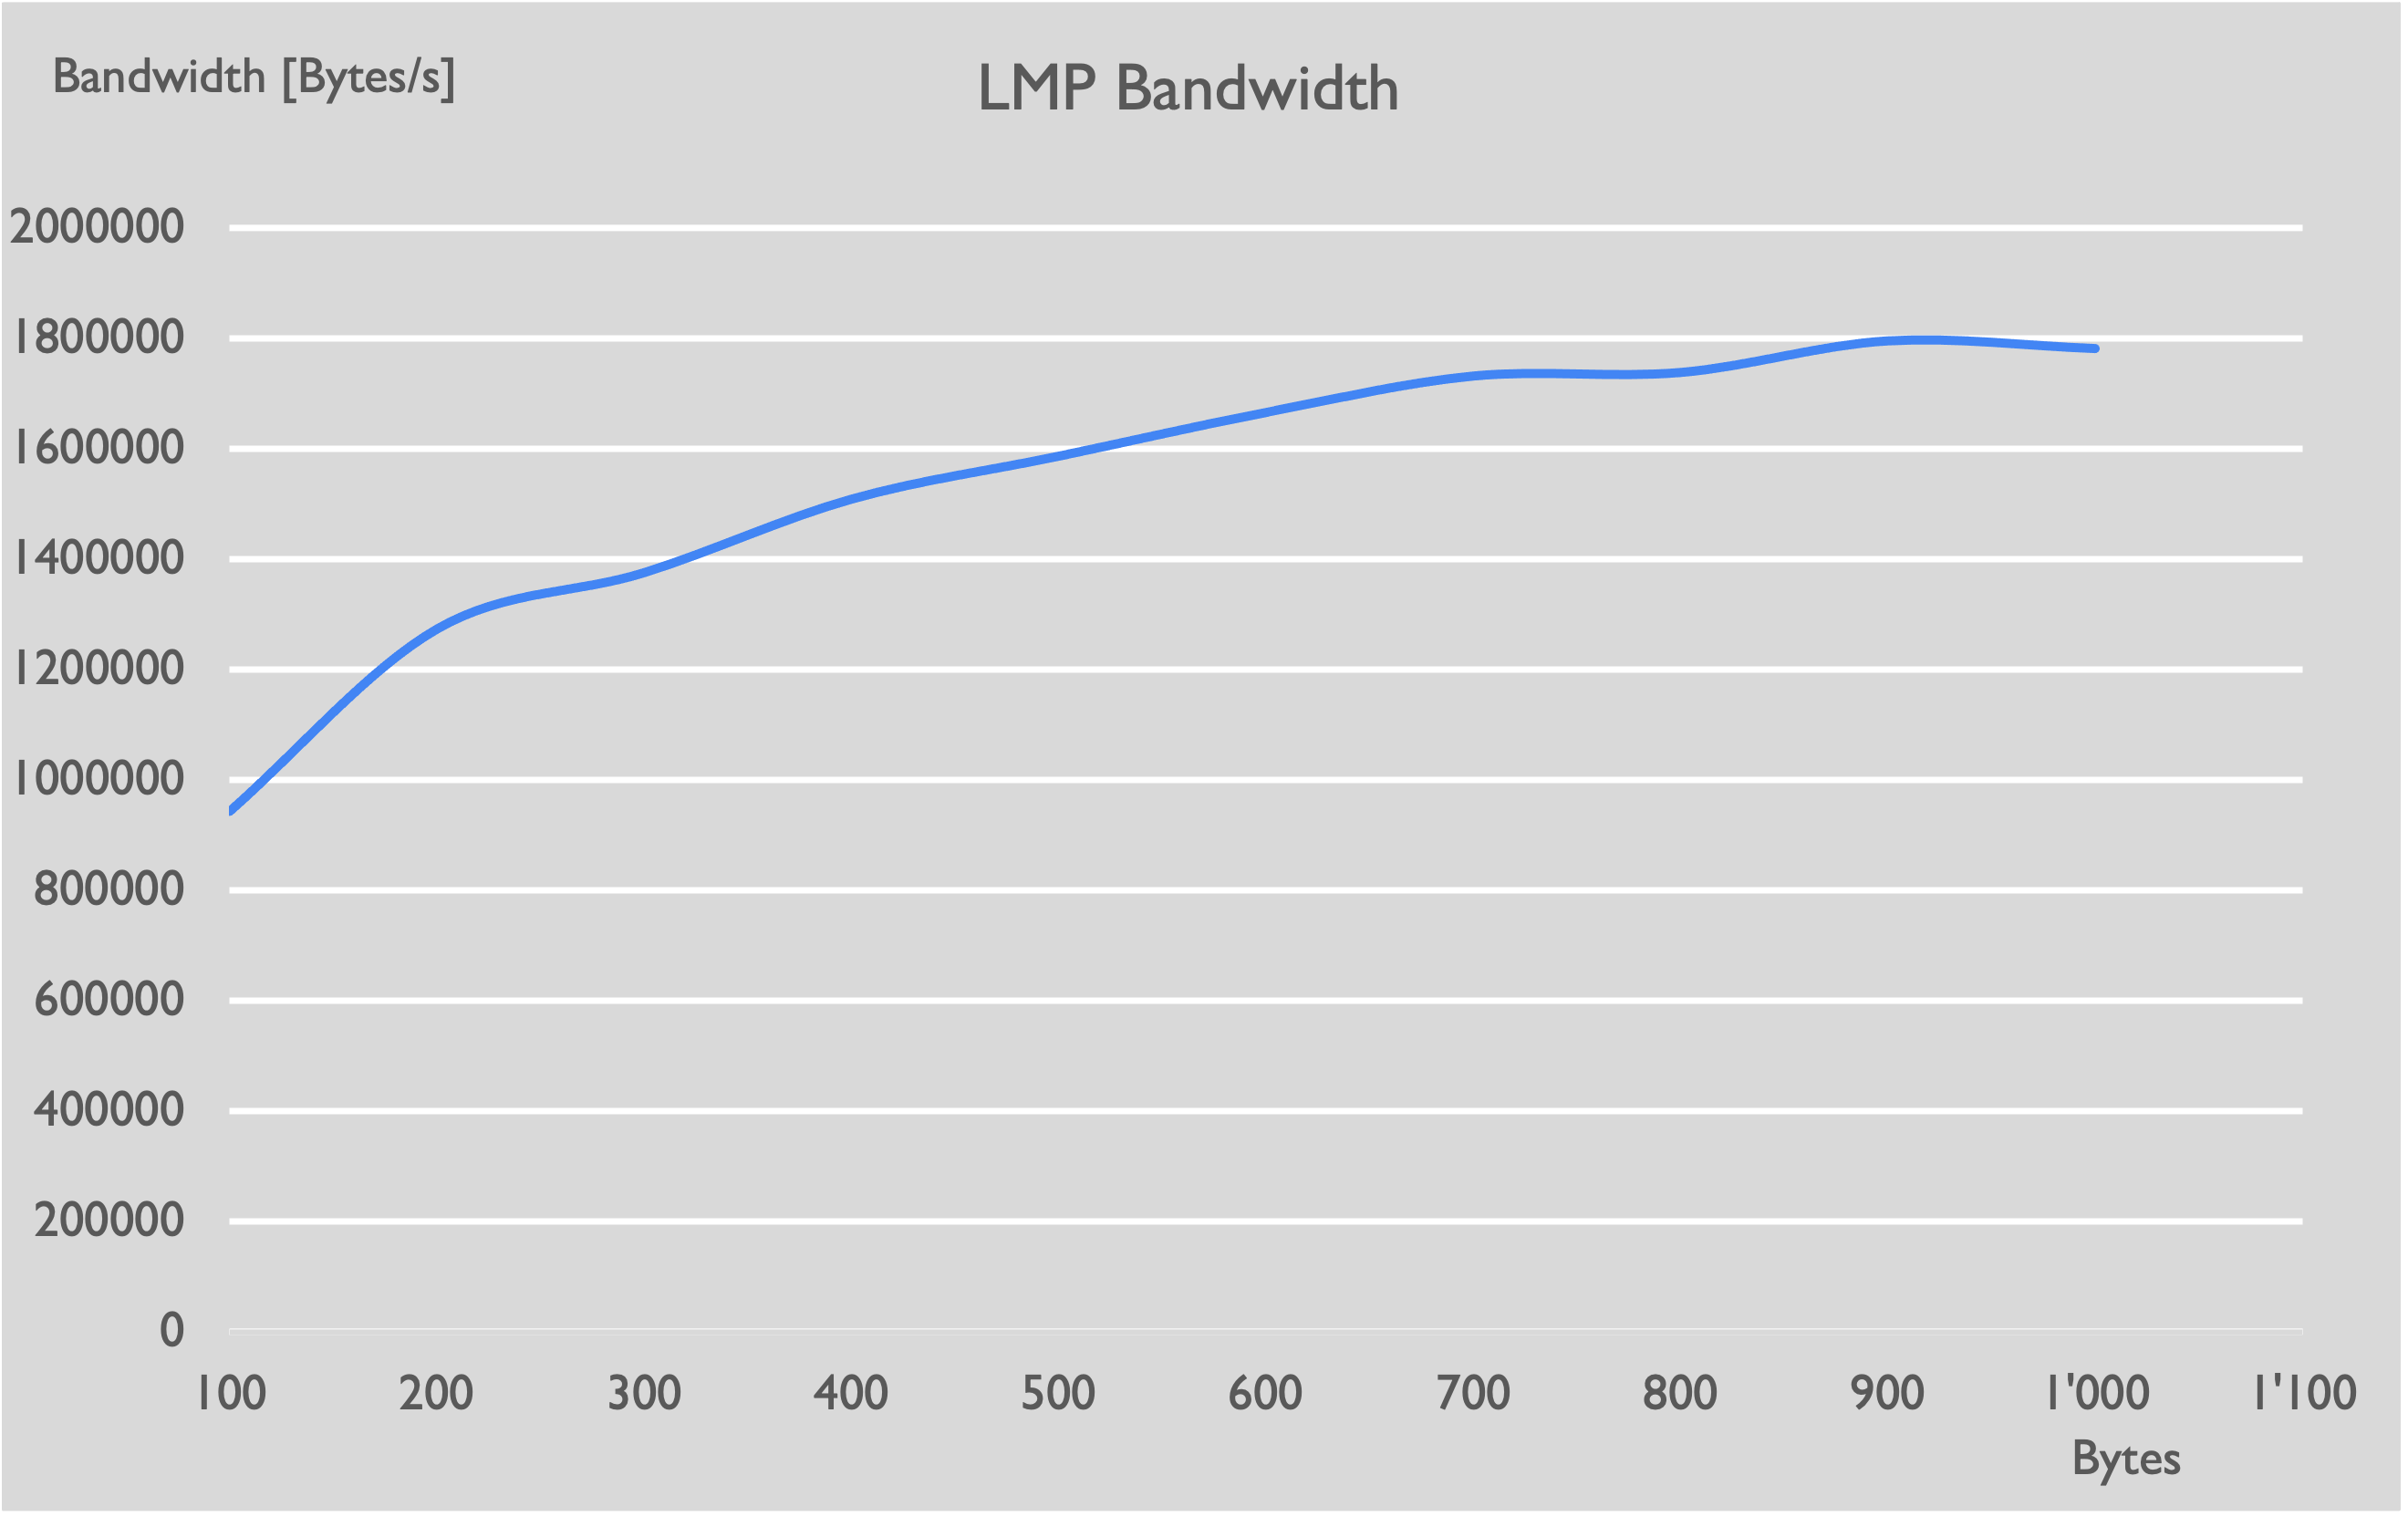
\includegraphics[scale=0.7]{lmp_bandwidth.png}
    \caption{LMP Bandwidth}
    \label{fig:my_label}
\end{figure}
As we can see, we reach transfer speeds of up to 1.8GB/s, which is roughly 10 times lower than the usual DDR3. The overhead of the first message which needs to be received can be seen by the lower bandwidth for smaller sizes, however the performance soon is saturated.

\section{Analysis} % Problems; performance; hindsight
Given more time, we would be interested to play with different packet sizes. As stated,
we currently use packets of 32 bytes. Benchmarking performance with other sizes 
would be a good idea. However, we weren't too concerned with this, since most of the RPC
messages we send (and crucially, the ones which are sent most frequently) fit into a single packet.

Another improvement would be to look at rewriting blocking reception of RPC messages,
which currently uses polling to check if an incoming message exists. As said, we 
abandoned the idea of using upcalls for receiving responses to blocking client requests due to race conditions 
which resulted from failure to abide by our stated invariants. Given more time, 
this would be a good performance optimization and a crucial improvement to our system.

Avoiding the idea of message-splitting altogether, 
using the shared-memory approach for dynamically sized messages could be 
analyzed further and performance compared. We suspect that starting from some size, 
sharing memory will outperform message-splitting substantially.


% extra:
% big messages
\chapter{Virtual Memory}
What should a virtual memory system provide? memory, safety, flexibility, efficiency
The next sections will describe how we achieved these goals.

\section{Memory Layout}
Central to this milestone was coming up with a useful layout for the virtual memory. To this end
we divided the virtual memory space available to user space (the lowest $2^{48}$ addresses on ARMv8)
into an unusable, a read-only, a heap, and
a stack regions. The unusable region is the page with the lowest addresses -- basically everything
that results in a segfault. Above that we have the read-only section where the code and all the static stuff %TODO: specify static stuff
is mapped.

The stack region grows down from the highest user space address. We made the design
choice to reserve a fixed amount of memory for each thread. This allows us not to worry
about stacks growing into each other and instead having a predictable stack overflow.
Currently, this value is set at 1 GiB per stack (i.e. thread), which is sufficient for our devboard.
However, for other platforms it can easily be increased as there is plenty of virtual memory.
Since the number of threads in Barrelfish is limited (see threads.h, currently 256), we
reserve the top 256 GiB for the stack region.

The heap region starts after the read-only section, which ends after 512 GiB and stretches all the way
up to the start (or rather end) of the stack region.

These sections are defined in \texttt{include/aos/paging\_types.h}.

\section{Allocating Memory}
In order to keep track of the address space, we reused our data structure that we used to track
RAM after some refactoring to have a common memory tracker interface (see subsection \ref{subsec:mm-tracker}.
For each of the three usable
regions described above we have a separate memory tracker to track which parts of the address space
have already been allocated. This allows us to reuse all the implementations for allocating, splitting,
and freeing of memory regions that we already had implemented for RAM.

By separating the management of virtual addresses for these regions into separate memory trackers,
we did not have to worry about the heap growing into the stack and vice-versa, as the respective 
memory tracker cannot hand out addresses for other regions than their own (given proper initialization).

It is important to note that requesting memory using \mintinline{c}{paging_alloc} would only allocate a free region
of virtual memory in the appropriate memory trackers. The behavior we settled on was that by default
\mintinline{c}{paging_alloc} would find free virtual addresses in the heap region as a wrapper around
\mintinline{c}{paging_alloc_region} where the caller can select from which memory region the free addresses should come.

These allocations of free virtual addresses are by themselves not backed up by memory. This is only
done once the memory has been accessed and a compulsory page fault has been taken.

\section{Handling Page Faults}
Once our system takes a page fault on a virtual address, the first thing the page fault handler does,
is check which memory region the faulting address belongs to. If it belongs to the unusable region
it goes ahead and throws a segfault.

Using the appropriate memory tracker we can now verify that the address we took a page fault on is actually
allocated. If it is not allocated, the handler again throws a segfault as only broken programs would try to
access memory without allocating some first.

If the faulting address is within an allocated region of virtual memory, the handler backs this address up
with actual memory by allocating a new frame the size of a page and mapping that fresh page at the appropriate
address in the page table. With this we are done with the handling of our page fault. Because we only
back up allocated virtual memory with a physical page once a page fault
occurs, we always round up the amount of requested memory to the next multiple of a page size. This way
we know that if we ever want to map a page to for a given virtual address and there is already a page
present, that the program must be incorrect and we can throw a segfault.

\section{Performance Analysis}
Throughout the project, we've found that page faults have been quite expensive. To verify this,
we measured execution times of our page fault handling.

\begin{figure}
    \centering
    \includegraphics[scale=0.65]{PageFaultHandling\_Latency\_Histogram.pdf}
    \caption{Page Fault Latency in microseconds}
    \label{fig:pfaults}
\end{figure}
Figure \ref{fig:pfaults} counts the frequency of page faults being handled in the given interval specified in the x-axis.
As can be seen in Figure \ref{fig:pfaults}, most page faults are handled in 2 - 4 milliseconds, while there
still are a few stragglers taking roughly 10ms. Stragglers can be explained by noting that sometime, 
slabs and slots need to be refilled, which increases the overall latency.

\section{Freeing Memory}
To free memory, we first identify the allocated virtual memory region the address belongs to.
Then we unmap all pages mapped for this virtual memory subspace and also free the allocation in the
respective memory tracker.

Our \mintinline{c}{paging_unmap} implementation walks all page tables in the identified memory region.
It unmaps all L3 page table slots in the region and also unmaps all L3, L2, or L1 page tables that might
be empty due to the unmap operation. Already free L3 slots are just left alone.

\section{Dynamic Stack Extension}
One extra challenge was the dynamic stack extension. Because of our separate memory trackers and the
code already in place, we were able to implement this quite easily. Whenever a new thread is started,
the initialization allocates stack space for that thread. Our implementation makes sure that the same
amount of memory (currently 1 GiB) is
allocated in the memory tracker for the stack region of virtual memory for every thread.

The fields \mintinline{c}{stack} and \mintinline{c}{stack_top} in the \mintinline{c}{struct thread} 
are then initialized to the appropriate boundaries of the allocated part of virtual memory. This allows
the function \mintinline{c}{thread_check_stack_bounds} to enforce the bounds of the stack at runtime.
Since this function is only called when a thread resumes, we also map the lowest page in the stack as
a guard page. Ideally, this guard page would be mapped with the guard flag on the page. Unfortunately,
it is not available on ARMv8 (at least according to the memory management code in the kernel). Thus,
we map it without any flag. This still does the job as a guard page as it will trigger a segfault if
any process faults on the guard page since it is already mapped.

With this setup, the stack is only ever backed by the least number of pages necessary, i.e. the pages
it already accessed.

\section{Challenges}
We faced some challenges implementing this milestone. The foremost was the problem of recursive
page faults, slab- and slot allocator refills. The problem of recursive page faults was fixed by
ensuring that the code path of handling a page fault does not incur a page fault. One example of such
a fix is that LMP messages of sufficiently small size (i.e. RAM capability requests) are constructed
in a static buffer before sending and upon receipt.

The problem of recursive allocator refills was a bit more tricky as it had a habit of coming back.
But the solution we ended up with is that all allocators keep a reserve of spare slots or slabs
such that they can provide resources for the process of refilling themselves. This invariant has to
be ensured at the proper place. For the slab allocators we do this at every instance before memory is allocated as to prevent 
the refill to be necessary during the allocation which would lead to recursive allocations. For the
two-level slot allocator we are using, we modified it to change to the other level when it still has
ten slots to spare. Because of the spare slots and the refill procedure that does not incur a page fault
there are no restrictions on the time when this can be done.

Another problem is the thread safety of all methods involved in self-paging. Multiple threads share
the same paging state and thus can and will cause bad interleaving in the paging methods. We opted
to curtail this problem by making the functions thread safe using locks. In the paging state, we added
a reentrant lock that locks at the beginning of functions modifying the paging state and unlocking
when that function is left again. This prevents any thread other than the thread holding the lock
from interfering with the progress of changing the paging state.

A small fun challenge was self-inflicted, because we wanted to malloc 1 TiB of memory. It turned
out that the malloc implementation in the handout still assumed 32-bit virtual addresses. Since
this is 2022 we changed the implementation to be 64-bitand succeeded in mallocing 1 TiB.

\section{Issues \& Limitations}
Our unmap implementation is terribly inefficient, since it needs to try and visit all page table
entries in the virtual memory region that is to be unmapped. When freeing our 1 TiB malloced buffer,
it took over ten minutes to try and visit all page table entries even though we only wrote three
bytes in the beginning, the middle, and the end of the buffer. However, we already had problems
implementing the current implementation. Therefore, we decided to leave it at that. However,
the page table walk could be sped up significantly by only visiting the pages that are actually mapped.


\section{Multi-core Support}

To use another core, we need to boot it, establish a communication channel between from the old core to the new core and define how memory management is done across cores.

In our system we make the assumption that core 0 is always present and only cores 1 to 3 are booted and shut down.

\subsection{Boot another core}

The main part about booting a core is allocating memory for various datastructures and passing these memory regions to the new core. Further, we need to tell the new core, where some fundamental binaries are such that it can execute them.

\subsubsection{Create the Kernel Control Block}

We start with the Kernel Control Block that needs to be allocated and retyped. At this moment it worth to be mentioned, that we always have to pass the physical memory address as opposed of a virtual one, such that the new core actualy know where that memory is. 

\subsubsection{Load the boot driver}

Next, we have to find the boot driver in the multiboot module and map it into our address space. As the boot driver is nothing else than a ELF binary we need to find the right entry point, in this case "boot\_entry\_psci". Then we also need to map the binary into our address space and get its physical address. Moreover, the bootdriver runs with a one-to-one virtual address to physical address mapping, so we have to relocate the ELF binary as well.


\subsubsection{Load the CPU driver}

The same has to be done with the CPU driver, but this time it is a different binary and with that also a different entry point to be looked for.

\subsubsection{Allocate the kernel stack}

The kernel needs its own stack, so we allocate 16 countinously aligned base pages and get their physical address.

\subsubsection{Loading init}

Also does the new core need to know what initial binary should be executed. Usually, that would be the "monitor", but as we do not have a "monitor" we use "init".

\subsubsection{Allocate kernel memory}

To load the init binary, the CPU driver needs some initial memory, that we have to allocate for it as well.

\subsubsection{Initialize the core datastructure}

At this point, we have all the ingredients to boot a new core. We only have to put all these information together in a compact and well know structure. That is the purpose of the core datastructure. It contains configuration parameters, locations and size of various memory regions we just allocated and the core ID.

\subsubsection{Flusing the cache}

To clean things up, we also need to flush the cache to make sure that all data we have just written is visible for everyone, including the new core.

\subsubsection{Spawning the core}

Finally, we can boot a new core by invoking the kernel capability.

\subsection{Communicate between cores}

The newly booted core needs to fundamental capabilities to work properly. These include a ram capability that represent a region of physical memory that it can manage for applications on its core, the bootinfo that contains also the multiboot module such that the new core can start other processes.
These capabilities are send over shared memory that is mapped in both cores. We discuss its communication mechanism further in the next chapter.

\subsection{Manage memory across cores}

We decided that every core should have its own memory that it can manage. For this, as we have four cores, a quarter of the memory on core 0 is allocated. The physical address of the capability representing this memory region is then send the new core, forged into a new capability and used to initialize the memory allocator.
Every core has a distinct PID range that it can use for spawning processes.

\subsection{Booting all cores and turning cores off and on}

We also implemented both extra challanges. Booting all cores was pretty straight forward, and we could easily reuse the same logic to boot core 2 and 3.
Turing a core off and then on again was a bit more involved and neede more digging. But in the end, we implemented a mechanism that allows core 0 to tell another core to turn itslef off. Turing a core back on involves the same steps as booting a core.

% allocate memory
% Create KCB & Coredata datastructures
% load the boot driver and cpu driver
% clean cache
% call spawn

% each core gets 512mb (core 0 initially has all memory and allocs for other cores)
% assumed core 0 is always present (only core 1-3 on/off)
% primary-secondary communication
% pid ranges per core

% extra:
% boot all cores 
% turn core off and on

\chapter{User-level Message Passing}

Communication between cores happens over shared memory. When a core is booted,
the parent core allocates some memory, maps it into its own address space and
provides its physical memory address and size to the child core. The child core
also maps this memory region into its address space, and now both core can
access the same memory region.

With this shared memory, both core, need to settle on a common communication
protocol such that they understand each other.

\section{Communication Protocol}

Each core can acts as a server or a client, that means it may react on incoming
messages or initiate messages to other cores.  We decided on having a
consumer-producer queue mechanism to exchange messages between two cores, with
the shared memory having the size of two base pages. 

We first implemented the communication protocol with a shared memory size of one
base page, but it turned out that messages, that are sent to a core as a
response to a request and messages that are sent to a core as a request, may
interleave. So we settled to have a shared memory of the size of two base pages
such that one base page can be used for server communication and one for client
communication. 

However, the communication protocol for both server and client is the same. We
will now explain, how two cores can communicate with each other over shared
memory of the size of one base page.

As already mentioned, the communication protocol is based on a producer/consumer
queue implemented with as a circular ring buffer. We need exactly two ring
buffers to communicate, as one ring buffer is for sending a message from on
core, and receiving on the other core. The second ring buffer is the same but
vice-versa, such that both cores can both send and receive messages. 

That means we need to split the base page once again into two equals parts. The
parent core will use the first half of the base page for sending messages and
the second half of the base page for receiving messages. The child core does the
same, but receiving on the first half and sending on the second half. Both cores
keep a pointer to an offset in the ring buffer to know where they should expect
the next message.

\section{Message Format}

Each message in our communication protocol is exactly 64 bytes, i.e. the size of
a cache line. That is important, such that we don't need to flush e message to
the memory, but it is enough to have the message in the cache, for the other
core to see it. This gives us a huge performance gain.

Each message has a header and a payload. The header contains metadata such as
the message type, the message state, payload size and if it is the last messages
in a chain of fragmented messages. The latter is important for sending messages
that are larger than 64 bytes, but more on that later. The header has the size
of exactly 3 bytes, and therefore there is space for 61 bytes of payload for
each message.

The most interesting header parameter is the message state. A message can have
three different states: created, sent or received. When a message is initially
created, it is marked as sent. When a message is sent from the sender's
perspective it is marked as sent, and it is marked as received from the
receiver, when it consumed the whole message.

\section{Sending and Receiving Messages}

To send a message, we need to get our current offset into the ring buffer, i.e.
a particular cache line. First, we check if the previously sent message over
that cache line is marked as sent in its header. If that is not the case, then
we filled the circular ring buffer completely and cannot send another messages
until the receiver has consumed some messages. However, if the message is not
marked as sent, but as received, then we can use this cache line to transmit
another message. We copy the message into the cache line, mark it in its header
as sent, and update our offset into the ring buffer to point to the next cache
line. The tricky part here is to deal with ARM's weak memory model. A weak
memory model does not guarantee that stores from one core are observer by
another core in the same order, that they are stored by the former. Luckily,
there are barriers to enforce, exactly that.

We need a barrier between checking for the message state and copying the message
in the cache line to ensure that we first check the state being received before
we overwrite possibly not yet consumed messages. And we also need a barrier
after copying the message into the cache line and marking the message as sent,
such that the message is actually written to memory before logically marked as
sent and consumed by the receiver.

To receive a message, it computes the current offset into the ring buffer to
know in which cache line the receiver should expect the next message. It  checks
repeatedly the message stored in this cache line for its message state. Once,
the message state is marked as sent, the receiver got a new message to be
consumed. To consume it, it is copying the content from the cache line, marks
the message as received and updates its offset into the ring buffer.

Again, we need barriers to make the whole receiving process work. Similarly, to
the sender, we need to insert a barrier before consuming a message such, that we
are sure that we first check the message state to be marked as sent before
actually reading its content. Also, we need another barrier between copying the
message content from the cache line and marking the message as received. The
same reasoning as above applies here.

\section{Sending large messages}

At this point, two core are capable of communicating with each other. But only
if the message, they would like to send, fit into a single cache line. We went
the extra mile and implemented the extra challenge fragmentation and reassembly.
For this we need to split the payload, that should be sent, into chunks fitting
into a cache line and reassemble them on the receiver side. Sending chunked
messages is pretty straight forward, but one point to mention here is the case
when we send many chunked messages and completely fill the ring buffer and hence
fail sending the remaining message. In this case, we implemented a linear back
off functionality that retries send the messages up to 32 times, such that the
receiver has time to consume messages and give space for sending the remaining
messages.

We decided to limit the maximal allowed size of messages sent over UMP to two
base page sizes. This way, we can allocate a temporary buffer on the receiver
side, that is guaranteed to contain the whole message after reassembling. The
receiver then simply needs to read all chunked message and reassemble them.

\section{Synchronous communication}

To provide synchronous communication over UMP we also added a function to our
interface that, sends a message and immediately tries to receive one, such that
we could offload this functionality directly into the library.

% maybe talk about server/client and binding

\chapter{Local Remote Message Passing}
\section{Introduction}
% give a short introduction into the problem, the goal, the approach,

\section{Designing Message Passing}
% Use cases: memory, init-comm, serial driver, between processes
% Either async vs sync -> easily usable for a server as well as for a client
% Choices: All using same channel. Locking -> where is concurrency possible
%          Separate channels for separate uses; also: how is state passed in messages
Local Remote Message Passing (LRMP), which is used to communicate between processes
on the same core is mearly a mean of communication. On top of such a functionality,
various designs can be implemented for allowing a safe, reliable and usable system
for communication. We will see in this chapter how we've built a system which allows
an easy integration for use in a Memory Server (to distribute RAM capabilities 
to processes),a Serial Server (for input/output to a screen) as well as an Init Server 
(for communication to the \texttt{init} process).

Of interest are the different choices one could use LRMP to communicate asynchronously and/or 
synchronously. Also, it's a big interest to utilize the asynchronous nature of LMP to
achieve high concurrency during operation. Lastly, while a functioning protocol for the basic
functionalities desired (communication with init, memory and serial servers) 
should surely be logically separated, there are many options one might separate them physically.
These can be isolated components over different channels, or handled by a single channel alltogether.

\subsection{Blocking vs Non-Blocking}
To embrace the non-blocking nature of LMP achieved through upcalls, we provide an 
easy interface for a process to register for the receival of such messages. 

\subsubsection{Non-Blocking}
For non-blocking communication, we focused mostly on the use-case of an arbitrary servers, 
which offers services to be received and processed in an endless-loop.

More concretely, any server (e.g. the memory server) can define a function which is to be called
on the receival of any LMP message through one channel. The interface of such a function looks like this:

% TODO TODO
TODO TODO

Using this API, a registered \texttt{handler-function} is reregistered on the receival
of each message. The only responsibility we give to the server is then to actively wait for 
messages to come in, which can be done in the all-to-familiar manner:

% TODO TODO
TODO TODO

\subsubsection{Blocking}
When talking about blocking communication, we talk about receiving messages we have mostly 
client-applications in mind. While a server usually only responds, a client requests.
In our cases throughout the course, these requests of clients made sense to be blocking, 
so that user-code only continues to run after a response has been received.

Blocking communication is achieved by polling on the channel until a message has been received.
As stated, having send-then-receive patterns in mind, we provide a call for doing 
both at once:

% TODO add aos_rpc_call signature
TODO TODO

We decided to wait for messages by polling on them, however we note that there might be 
alternative designs which avoid polling on a response. 

In an older design, we implemented blocking communication by receiving the message asynchronously 
by registring a receive handler handler and just waiting for a response 
using \texttt{event\_dispatch()} again.
However, due to race conditions between different client calls, we abandoned this idea 
for the time being. 

We're still convinced that this improvement would have lead to a performance increase in 
our implementation, especially under heavy load.

\section{Lifetime of a Channel}
% binding; registering; closing
Before using a channel, it needs to be created. 
In our case, we needed to create a channel between the \texttt{init} process and a newly-spawned
child process. After the channel has been established between the two parties, 
it can be used for communication. In the following, we describe the setup (binding) 
and teardown (closing) of a channel.

\subsection{Binding}
Let's have a look at the init server.
When a new child process is spawned, the \texttt{init} process hands it an endpoint-capability
to itself. That way, the child already knows to which channel it needs to bind. 
Given that capability, the child has enough information to contact \texttt{init}, and 
\texttt{init} has enough information to receive messages. To also allow \texttt{init}
to send to the child, the child process will create a new endpoint and send it to \texttt{init}
in a binding handshake. Using this endpoint, both parties can then send and receive.

\subsection{Closing}
% TODO
TODO TODO

\section{RPC State}
During operation, we support sending messages of dynamic size.
Supporting the option to send messages without causing page faults was crucial 
to us. Besides increased performance, it's is also necessary for using RPC 
during page faults. Since during a page fault, we need to guarantee that no 
nested page fault occurs, we added a static buffer to each RPC channel of 4096 bytes, 
which is used to send statically sized RPC messages that fit into it.
That way, functionality like sending RAM over RPC can use a already-mapped for 
receiving messages, thus avoiding page faults. In general, any established 
RPC channel has the following structure:

% TODO graphic
% graphic contains: RPC channel, pointer to a static buffer, pointer to a dynamic buffer
TODO TODO 

Besides the static buffer that every RPC channel has, one can also send 
dynamically-sized messages, which are contained in another buffer.




We now describe the state which is kept by our RPC communication protocol.

\subsection{Message Sizes}
We support sending messages of dynamic sizes. To achieve this, we considered 
either shared memory or breaking messages into smaller packets.
While shared pages will decrease the overall LMP-traffic, we would also 
require additional logic for sharing the pages necessary as well as 
copying a potentially large source buffer to this large memory region.

Many questions arise:
\begin{itemize}
    \item Who has read/write access to the shared page? 
    \item When is this shared page unmapped?
    \item At which size of payload will shared memory make sense?
\end{itemize}
On the receiving side, the data would need to be copied out of the shared region 
into newly allocated memory. The copying is necessary since the sender 
might want to unmap the shared memory region at some point and it shouldn't be 
the case that both processes modify the same shared memory region.

Splitting messages into multiple parts has a very straight-forward structure 
without having the additional bookkeeping complexity shared pages have.


In the end, we decided to use the message-splitting approach.
More precisely, any message packet we send over LMP is sized at most 32 bytes
large.  
% TODO evaluation
TODO TODO

\subsection{Message Structure}
Below, we describe the structure of a whole message of dynamic size.
\begin{lstlisting}[language=C]
struct aos_rpc_msg {
    aos_rpc_msg_type_t type;
    char *payload;
    size_t bytes;
    struct capref cap;
};
\end{lstlisting}
Every message sent over an LMP channel contains a message type determining 
the type of request, the actual payload, payload size and optionally, 
also a capability to be transfered through the channel. 
Additionally, to the beginning of a message to be sent, we prepend its size 
to the payload. That way, the receiving size can determine the size of an 
incoming message and knows how many more are to be expected.

\subsection{Invariants}
To achieve thread-safety, our LMP communication protocol 
follows the following invariants:
\begin{itemize}
    \item Client send-receive patterns are atomic with respect to the channel
    \item Server receive-send patterns are atomic with respect to the channel
    \item No process uses a channel as a server and client at the same time
    \item TODO
\end{itemize}
These invariants allows us to avoid race conditions and the guarantee that 
when a client receives a response, it will be the response to the the client's
request and not the response to any other request from another thread.
To achieve that, it's also necessary that no process uses a both server and client, we never 
With that at hand, we have a total order of RPC requests of a client and no 
reponse-mixups.

Note at last that these invariants are only concerning a single channel.
Different channels follow no requirements with respect to other channels 
and can be treated separately.

\section{Implementing Functionality on Top of LRPC}
Now that the structure of single LRPC-channels have been explained, 
lets have a look at how they are used to build actual services and how 
they interleave at the example of our memory, terminal and init servers.

\subsection{Physical Separation of Services}
We decided to separate the memory server from the init server.
This has been crucial, since by our invariants, send-receive and receive-send 
patterns must be atomic. Thus, we can't allow an RPC call to 
start recursive RPC calls (breaking atomicity). Since dynamically-sized messages 
need to allocate dynamic memory when receiving an arbitrary-sized response, 
it could otherwise happen that memory is requested during an RPC call.
This could (and did) lead to recursive page faults.

Separating the memory server completely fixed this issue.
The two channels are set up for each new child process and go from the child to the 
\texttt{init} process and use the same waitset.

\subsection{Memory Server}
The memory server runs on the \texttt{init} process and receives RAM cap requests.
Since these requests and responses are all statically sized, no recursive page faults 
happen. Since our interface allows sending/receiving capabilities, this 
is already enough to implement the memory server.
Similar to the \texttt{init} server, it performs a handshake with the child process
when it is spawned. 
\subsection{Terminal Server}
% TODO
TODO not init right?
\subsection{Init Server}
% TODO
The init server registers the following handle-function 
\begin{lstlisting}[language=C]
    errval_t init_process_msg(struct aos_lmp *lmp)
\end{lstlisting}
It is responsible for handling spawn-requests, sent strings/numbers, PID lookups to receive 
the name of a process given its PID, and clients can also request to receive a list of all PIDs.

All requests to this service are stateless - all information for a request must be 
contained in the request itself.


\section{Encountered Problems}
We had a few problems with our initial RPC implementation, 
which after some revisions led to the invariants stated above. Some of these problems were:
\begin{enumerate}
    \item Mixing server and client functionality led to race conditions.

    \item When implementing support for page faults, we realized that it must be possible 
to guarantee that a RPC call will cause no recursive page fault.

    \item When mixing LRPC with URPC, it has become crucial to abstract LMP and UMP as much 
as possible, to avoid a confusing interface for a programmer in user-space.
\end{enumerate}

\section{Analysis} % Problems; performance; hindsight
Given more time, we would be interested to play with different packet sizes. As stated,
we currently use packets of 32 bytes. Benchmarking performance with other sizes 
would be a good idea. However, we weren't too concerned with this, since most of the RPC
messages we send (and crucially, the ones which are sent most frequently) fit into a single packet.

Another improvement would be to look at rewriting blocking receival of RPC messages,
which currently uses polling to check if an incoming message exists. As said, we 
abandoned the idea of using upcalls until a message is received due to race conditions 
which resulted from failure to abide by our stated invariants. Given more time, 
this would be a good performance optimization.

Avoiding the idea of message-splitting alltogether, 
using the shared-memory approach for dynamically sized messages could be 
analyzed further and performance compared. We suspect that starting from some size, 
sharing memory will outperform message-splitting substantially.


% extra:
% big messages

\section{Shell}

The shell is split into two modules, a serial server and the shell itself.

\subsection{Serial Server}
The serial server can be seen as a rudimentary TTY. It reads and writes through UART and buffers incoming characters.
With only little modification multiple TTYs could be launched, each using a different UART port.


\subsection{Shell}


\chapter{Filesystem}

\section{Introduction}
For the filesystem, we support SD-cards running FAT32. The filesystem we've implemented 
is built as a service, exposing RPC calls for file operations like opening, closing, writing, reading, etc. 
to user processes, which then can be called by the usual libc functions like \texttt{fopen}, \texttt{fclose}, \texttt{fwrite}.

The alternative, which is building the filesystem as a library, has not be chosen because the filesystem as a service 
gives in our eyes a better abstraction to the underlying FAT32 operations. Another reason why we chose the filesystem as a service
is because it does decrease RPC communication, leading to overall better performance.  

\subsection{Operations}
The operations implemented as a service over RPC calls are:
\begin{itemize}
    \item \texttt{aos\_rpc\_fs\_open}: Open a file with given flags
    \item \texttt{aos\_rpc\_fs\_close}: Close a file
    \item \texttt{aos\_rpc\_fs\_create}: Create a file
    \item \texttt{aos\_rpc\_fs\_read}: Read open file contents into buffer
    \item \texttt{aos\_rpc\_fs\_write}: Write buffer contents to a open file
    \item \texttt{aos\_rpc\_fs\_lseek}: Seeking in a file
    \item \texttt{aos\_rpc\_fs\_dir\_action}: Used to perform the two operations \texttt{mkdir}, \texttt{rmdir}
    \item \texttt{aos\_rpc\_fs\_readdir}: Read directory contents
    \item \texttt{aos\_rpc\_fs\_fstat}: Get file status
\end{itemize}

\section{Block Driver}
After flashing a new filesystem onto the SD-card, we can communicate with it over 
the block driver over the process \texttt{fs}, which has access to the devframe necessary
for using the driver. Since it's the only process with access to the SD-card, we don't have to worry 
about concurrent read/writes in the filesystem.

\subsection{Performance Improvements}
To improve the block driver, we note that we always only read/write blocks of the 
same size with it. Thus, it's enough to only set the block-size once in the beginning,
instead of setting it every time we read/write a block. As we will see during the 
performance analysis in the next section, this will already give a 2x speedup.

There are many other performance improvements which could be made.
Very interestingly to me with respect to FAT32 is that reading/writing whole 
clusters at once could be done much faster. As can be seen in the next section,
sending commands over the block driver alone will take a lot of time, 
so reducing the number of commands sent to the block driver can be of essential 
importance for performance.

It's also possible to read/write specific block-lengths with each write.
However, this change in block-lengths needs to be communicated to the device,
thus another command needs to be send to the SD-reader. We immediately see 
that this constitutes a tradeoff between send-commands and DMA-access time.
While always reading large blocks has few send-commands, DMA over large memory 
takes longer than for small blocks. It could have been interesting to also 
check if or at which point it makes sense to work with variable-sized read/write 
commands.

As a last possibility for improving performance, it could have been possible 
to fetch information from the SD-card to obtain more information of frequencies 
which could be used to allow for faster access speed.

\subsection{Performance Analyis}

\section{FAT32 Implementation}

\subsection{Assumptions}
We assume we receive a valid FAT32 filesystem. We thus don't do any additional 
checking/fixing/infering of the filesystem present.

\subsection{Abstractions}
Wherever possible, we tried to abstract away sectors as much as possible.
Instead, we focused on clusters and indeces into clusters, so that 
we wouldn't have to worry too much about cluster traversals in terms of 
sectors, where in which cluster we are, etc. Seeing FAT32 as a linked-list 
of clusters is much easier than seeing it as a linked-list of sector-arrays.

For buffers which we use to read/write to, we introduced 
\begin{lstlisting}[language=C]
struct phys_virt_addr {
    // physical address of memory segment
    lpaddr_t phys;
    // virtual address of memory segment
    void *virt;
    // last sector read/written
    uint32_t last_sector;
    // is the buffer dirty?
    bool dirty;
};
\end{lstlisting}
we use it to keep track of where we read/write to. The last two members 
are important for caching, which will be explained laster.




\subsection{Caching}
One file write/read can potentially look at one FAT-sector multiple times,
or could write to the same data sector multiple times. Since every 
read/write from/to a sector on the SD-card is very expensive, a big 
performance increase was the idea of caching reads/writes to the disk.

In a first attempt, we never performed a read from the SD-card if 
the last read/write to/from the SD-card was to the same sector. This can 
be pretty easily by just remembering the last sector each time.

A next observation was that there is much locality in a directory-entry 
as well as a FAT-sector, since many requests looked at closed-by indeces
of a sector. For that reason, we decided to use a different buffer 
for storing any read/writes to a data-sector and a different one for 
FAT sectors (and directory-entry-sectors). 
A write would still always write, it is write-through.

Using these two different buffer, we benefit from locality.
To extend this idea even further, an LRU-approach with $N$ different 
buffer would lead to even fewer reads from the SD-card.
TODO

\subsection{Limitations}
Due to time-constraints, no support for timestamps or read-only files is implemented.
Also, no estimates of free clusters are used.
\section{Filesystem Implementation}
To implement the filesystem, we tried to keep the original approach of \texttt{ramfs}
as much as possible and replaced functions like \texttt{ramfs\_open}, \texttt{ramfs\_close}
have been replaced by \texttt{aos\_rpc\_fs\_open}, \texttt{aos\_rpc\_fs\_close}.

We store a opened file in a simliar struct as in \texttt{ramfs}:
\begin{lstlisting}[language=C]
struct fat32fs_dirent {
    char *name; 
    size_t size; 
    bool is_dir; 
    // cluster containing the directory-entry
    uint32_t dir_cluster; 
    // index into that cluster
    uint32_t dir_index; 
    // first data cluster of file
    uint32_t start_data_cluster; 
};

struct fat32fs_handle {
    int flags;
    // unique id of the opened file
    fileref_id_t fid;
    domainid_t pid;
    char *path;
    struct fat32fs_dirent *dirent;
    union {
        uint32_t dir_offset;
        uint32_t file_offset;
    } u;
    // current data cluster as 
    // specified by dir_offset/file_offset
    uint32_t curr_data_cluster;
};
\end{lstlisting}
Of particular importance is the member \texttt{fid}.
This ID is a unique ID under all the opened files in the filesystem 
which is used to identify an opened handle. Any RPC request to an opened
file identifies the handle uniquely by this FID.

In the \texttt{fs} process, the following happens when a new file/dir is opened:
\begin{itemize}
    \item Create new handle, store file-info into it.
    \item Assign new unique FID to handle
    \item Add into hashmap: FID $\Rightarrow$ Handle 
    \item Append to hashmap: Path $\Rightarrow$ Handle
\end{itemize}
The first of the two hashmaps is used to find the handle of an opened file by FID in constant 
time. The other stores all FID's which have the same file opened. Using this second hash map,
we resolve many thread-safety issues, which will be explained later.

\subsection{Service}

\subsection{Thread Safety}

\subsection{Security}
For a full-blown OS, it makes sense to have a security layer in place which 
doesn't allow for one process to read/write using FID's of another process.
This could have been done in multiple ways. One could be to authenticate the RPC channels,
so that every FID is also linked to a specific channel. That way, requests to foreign 
FID's could be rejected. This could also have been done with special capabilities to
any opened file/directory. 

As this feature was of rather low priority given the problems we had mentioned
during the integration, no additional security feature was implemented.

\section{ELF Loading}
Due to the problems during integration-phase, we didn't have time to implement
the ELF loading feature.

However, for the sake of completeness, we now state how this would be achieved.
Given our existing code, the approach we would follow is to use 
the file system to load the complete file into memory. After that,
any arguments to the program would be passed to by the shell.
To actually load the in-memory program, we can use existing functionality 
we have in our \texttt{spawn} library, where multiboot programs 
are also loaded into memory. After this step, we would start the program 
in the same way as we did for any other program.

\section{Performance Analysis}

\section{Issues}
\chapter{Nameservice}

TODO
\chapter{Networking}

\section{Access the hardware device registers}

The network process runs as a standalone process in user space. Therefore, it
needs to have access to the Device Frame capability that grants accesses to the
hardware device register. This was the starting point for this individual
project. We decided to pass the Device Frame in an arg cnode slot as it is
proposed in the manual. For this to work, we also needed to change the interface
of our spawn.h as currently we only could set up and dispatch the whole process
in once. But by having to provide a capability in a cnode slot we had to cut
those to parts into two, such that we could set up the process first, include
the capability in the arg cnode slot and only then dispatch the process.  The
corresponding part in the network process was significantly easier. We only
needed to map the capability in the arg cnode slot in to our virtual address
space.  Once, that was done, we could properly set up the network driver and see
the first packets arriving at our interface.


\section{Safe Send Queue}

For sending and receiving packets, the network driver has to communicate with
the hardware device.  The network driver works with two queues: the receiver and
the sender queue. If we want to send a packet, we have to warp it in a buffer
and then provide it to the sender queue. Those buffers cannot be at any
arbitrary place in the memory, but have to be in a region that has  been
registered beforehand with the queue.  As stated in the manual, it is important
to not enqueue two buffers that are stored at the same location in the region
twice before dequeueing. This is because,  every buffer has an owner, either the
network driver or the hardware device, and would result in undefined behaviour.
With this in mind, we developed a safe queue that provides an interface to place
some data in the sender queue. The safe queue simply keeps track of free buffers
in the region registered with the underlying sender queue. That means when we
want to enqueue a packet in the sender queue, we pass the packet to the safe
queue, and it will do some sanity checks, get a free buffer, copy the packet
into the free buffer and then enqueue the buffer into the sender queue, marking
the buffer as used.  There is no dequeue interface for the safe queue, but
somehow the buffers, that have been processed by the hardware device and are now
again owned by the network driver, have to be dequeued and marked as free
buffers again. This is done on every packet that is sent. While getting a free
buffer for the sending packet, the safe queue also dequeues all possible buffers
from the sender queue, such that we don't run out of free buffers.

The receiver queue, on the other hand, is much easier to handle. Here, we simply
dequeue a buffer that contains an incoming packet, extract the packet, pass the
packet to the packet handler of our network stack and then enqueue the buffer
again.

\section{General Receive Flow}

Upon receiving a packet, the packet is passed to a single point of entry, namely
the packet handler of our network stack.  The packet handler parses the packet,
determines the type of the packet, and passes it to more specialized handlers.
We implemented the handling of ARP packets and IP packets and with that
corresponding handlers.  While the ARP packet is already completely unwrapped,
the IP packet has to be parsed further, the type has to be determined again and
then has to be passed to another set of handlers. In this case, it may be an
ICMP, IGMP, UDP, UDPLITE or TCP packet type. We only implemented handlers for
ICMP and UDP packets.  Once a packet is completely unwrapped, it may be
processed correspondingly. That usually includes doing some legitimation checks,
storing the contained data, and may even trigger an immediate response. We
discuss this further in the upcoming sections.

\section{General Send Flow}

When we want to send data to another host, we first need to wrap that data into
a network packet. That may include several layers, depending on the type of data
we want to send. For this purpose, we implemented a packet assembler that is
capable of doing exactly that. Our packet assembler support assembling ARP, ICMP
and UDP packets. The assembled packet can then be enqueued in our safe sender
queue, ready for transmission.  Creating a convenient implementation for
assembling packets was a bit challenging. While the layering aspect of a network
stack is well known and also implemented in our packet handlers, it is a bit
harder to implement for packets assemblers than we initially thought. For
example, the final UDP packet has be in a continuous region of memory, starting
with the Ethernet header, then the IP header, then the UDP header and finally
the UDP payload.  If we want to follow the layering approach, then we would have
to first create the UDP packet, wrap it in a IP packet and finally in an
Ethernet packet. But as we start logically with and UDP packet, the memory
region starts with an Ethernet packet. So, either we have to allocate space for
the whole network packet, when we allocate the UDP packet or only allocate space
for the UDP packet, pass is to the next lower layer, where we allocate space for
both IP and UDP packet and copy the UDP packet from its previous memory region.
We even checked out the Linux network stack implementation for inspiration.  In
the end we chose our own, at the moment, convenient approach.  We provide packet
assemblers for ARP, ICMP and UDP packets, and each returns the final, completely
assembled packet. For example, the UDP packet assembler allocates space for the
whole packet including the Ethernet header, the IP header, the UDP header and
the UDP payload. It then starts filling the packet with data from the start of
the packet: first the Ethernet header, then the IP header, then the UDP header
and finally, its payload. This may not be the most scalable approach and may
introduce complication, when one wants to extend the network stack with new
layers or similar, but was at the moment of implementation the simplest way to
get started, so we kept this style for the all packet assemblers to be
consistent.

\section{ARP}

The address resolution protocol (ARP) is necessary to resolve a given IP to its
MAC address. This mapping is then stored in the ARP hash table for future use.

There are two possible types of ARP packets that our network stack may receive:
ARP requests and ARP responses. 

ARP requests arrive when anyone in the network wants to know the MAC address to
an IP address. So if the IP address is not our, we simply ignore the packets, as
we should not answer that request. On the other hand, if it is our IP address,
then we have to assemble an ARP packet that contains our MAC address and send a
ARP response to the original sender. At this point, we also store the IP to MAC
mapping in our ARP table such that we don't have to resolve this IP in the
future.

But if we don't know the mapping, we have to ask for it. Here, we assemble an
ARP request packet and broadcast it on the network, so that the owner of the IP
address may respond. When we receive it, we store the mapping in our ARP table.
At this point, we have to deal with the asynchronicity of the network. We need
the MAC address to continue, but also don't know when we will get the response
from the owner of the IP address.  Here, we tried two different approaches to
resolve an IP to a MAC address if we don't know the MAC address already. One was
to send the request and then wait for a given amount of time for the response
before returning an error. The other was to send the request and then
immediately return an error, implying that the caller has to handle that case
and to retry the resolution. We implemented the former approach.

\section{Ethernet}

This layer is relatively easy to implement. When we want to wrap an ARP or IP
packet into an Ethernet packet, we only have to prepend an Ethernet header
containing the source and destination MAC address and the type of the contained
data, i.e. ARP or IP.  Reception is also easy, as we only need the Ethernet type
to determine whether we have to call the ARP or IP packet handler.

\section{IP}

Assembling an IP header is also pretty straight forward with our assumptions we
have taken. Those include, we only assemble IPv4 packets, set the TTL to 128
only send IP packets that should not be fragmented.  Those assumptions also
simplify the handling of an incoming IP packet. We only process IPv4 packets
with a valid checksum and at least have the size of an IP header, and drop
fragmented IP packets. Based on the protocol, we then call the ICMP or UDP
handler, that we have implemented. All other protocols are not implemented, and
those packets are dropped.

\section{ICMP}

To successfully ping the Toradex board from another host, we have to reply to
valid ICMP echo requests with ICMP echo replies. An ICMP packet contains an
Ethernet header, an IP header, an ICMP header and some payload. With creating
the Ethernet and IP header as described above, the only part missing is the ICMP
header. Creating the ICMP header includes setting the ICMP type to echo replies,
the code to 0, the ID, sequence number and payload to the values that were
provided in the received ICMP echo packet and finally computing the check over
the ICMP header and payload. With that, we were able to ping our Toradex board
from our laptop!

On the other hand, we also wanted to ping other hosts from or Toradex board. So,
we have to be able to send ICMP echo requests and with that, we had to figure
out the meaning of the ID, sequence number and payload parameters.  As we know,
the ICMP serves the purpose of transmitting information and errors about the
IPv4. We are initially quite puzzled how an application, in this case "ping", is
able to receive incoming ICMP packets, as ICMP does not know the concept of
ports, therefore the well known demultiplexing process from UDP and TCP is not
possible here.  It turns out, that if one runs multiple "ping" instances on a
host, all "ping" instance get all ICMP responses and have to figure out which
one are responses to own requests. This is done with the ID parameter. We
decided to set the ID to our process number to distinguish the responses. We
also inspected how the real "ping" (i.e. the own installed on my laptop by my
package manager) chooses its ID and interestingly, it's not the process ID but
the value of a counter that increments with every "ping" instance. So, somehow,
every "ping" instance knows how many instances it is.  If you ever run the
"ping" command, you know that per default "ping" periodically send ICMP echo
packets to the provided host and reports the latency for each one until it is
terminated. As responses may arrive out of order, "ping" somehow needs to map
the response to the original request, and that is what the sequence number in
the ICMP header is used for.  Finally, ICMP packets may contain a payload and
under the hood "ping" puts random data into an ICMP echo packet and check if the
corresponding ICMP echo reply packet contains the same data and reports an error
otherwise.  This was an interesting part of building the network stack, as
"ping" is such a natural tool to use, one does not really think about its
internals.

With ICMP not knowing the concept of ports, we were also puzzled how we should
actually provide a ping instance with incoming ICMP packets. As we see in the
next section about UDP, every app has its socket with its own queue of incoming
packets. In the case of UDP, it is clear that every process has its own socket
and therefore it is straight forward on how the demultiplexing happens. In the
case of ICMP, it was not that clear. First, we had exactly one socket with one
queue that holds all incoming ICMP packets. But if we have two processes
consuming from the same socket, then packets intended for one process may be
consumed by the other, that simply ignores it and vice versa. So, we introduced
a queue for each process that want to consume ICMP packets and hence every
process gets every ICMP packet and has to do the demultiplexing in the process
itself, as it is intended. This of course brings a lot of packet duplication
with it. In the end we had also ICMP sockets like UDP socket, but here, they are
not distinguished by port, but by the process ID. 

\section{UDP}

We approached the implementation of UDP by setting up a UDP echo server directly
in the network stack. Therefore, if a UDP packet arrives at the UDP handler, we
immediately assembled a UDP packet and sent it back to the sender contains the
same payload. This allowed us to focus on assembling a UDP packet and setting up
the UDP header appropriately. Namely, a UDP packet contains an Ethernet header,
an IP header, the UDP header and the UDP payload. The UDP header contains the
source and destination port and the total length of the header and payload.  But
we had a major drawback here: we could not make the checksum work. Somehow, the
bytes representing the checksum in a UDP header were different when parsed on
the board and when inspected in Wireshark in the same packet. All other bytes
around the checksum matched, i.e. source and destination port, length, payload,
but not those representing the checksum. We had no idea why this would happen
and as UDP checksum is not mandatory in IPv4, we simply skipped that part for
both sending (creating the checksum) and receiving (verifying the checksum).
Once, we were confident with implementing the UDP correctly, we started
implementing UDP sockets. This is needed to demultiplex incoming UDP packets
based on their destination port to the corresponding client application that is
listening on that port.  A UDP socket is simply a producer/consumer queue. When
a UDP packet arrive in our network stack, the right socket is found based on the
port and its payload along with some needed meta information such as the source
IP and port is placed at the producer size of the queue. The client application
is then responsible to repeatedly poll this queue for new packets to consume.
This polling functionality is provided by the network service, describe in the
section below.  Other functionalities provided to the client application are of
course first creating a socket and also sending over the socket. It is now
allowed to have two UDP sockets listening on the same port, and therefore this
is checked in the socket creation. All existing UDP sockets form a simply linked
list and therefore new UDP socket are appended to this linked list. Sending over
a socket is putting already known parts together, such as getting the MAC for an
IP, assembling a UDP packet and putting it into our safe sender queue.

\section{Debugging}

The main tool in use to debug our network stack was Wireshark. It gave us
confident that the packets, our network stack is sending, are correct, as
Wireshark was able to parse it. Also, the other way around it helped a lot,
knowing what an incoming packet contains so, we could set up our handlers
correctly.

Other tools we used to trigger the correct path in our network stack were
"arping" to send a ARP request to the Toradex board, "arp" to check the ARP
table on the host to ensure that our network stack provided the correct MAC
address, "ping" for ICMP echo packets, "nc" both as a UDP client and UDP server
to test the sending and receiving functionality of UDP packets in our network
stack.

Further, we implemented debug print functions for every packet type (Ethernet,
IP, ARP, ICMP and UDP), the ARP table, IP and MAC addresses and also the
producer/consumer queue in our sockets to have some insights of what is
happening in our network stack.

\section{UDP Hack}

While implementing the UDP part in the network stack, we had to apply some hacks
to test the functionality. One was already mentioned above, by echo UDP packets
directly in the network stack.  Another one, to test the reception of UDP
packets from the client application's perspective, that means consuming the
packets that are stored in the producer/consumer queue in a UDP socket, we
proceeded as follows. Upon reception of a UDP packet in the network stack, we
stored the UDP packet as described above in a UDP socket, but then immediately
consumed it over the same interface that would a client application use to
receive a UDP packet and also send some payload back over the interface. This
required of course to create a UDP socket statically at the setup of the network
process, to make the UDP handler not drop the packet.

\section{ICMP Hack}

The UDP hacks described above are quite straight forward. Testing the ICMP part
is a bit more involved. Responding to ICMP echo requests required no hacks, as
it can be directly testing by using "ping" on another host.  But issuing own
ICMP echo requests is trickier. At this point, we have not yet implemented our
own "ping" and also do not have our nameserver setup yet. So communication
between any two processes is not yet implemented, hence we had to apply another
hack to make this work directly in our network stack: Upon handling a ICMP echo
request, we do not directly return, but send our own ICMP echo request to the
host, that just pinged us with some dummy ID, sequence number and no payload and
then try to consume an ICMP echo reply over the ICMP socket like a client
application. On the first try, consuming the ICMP echo reply will fail, as the
request has not yet made the whole roundtrip to the host and back. When we send
another ICMP echo request from the host to the Toradex board, we are going to
again handle it, issue our own ICMP echo request, but at this consuming from the
ICMP socket will not fail, because the ICMP echo reply from our previous ICMP
echo request, will be stored in there. This way, we can then check if the ID,
sequence number and payload align with our dummy values.

\section{Network Service}

Such that other processes, like multiple UDP servers, can use the network stack,
we need to expose our network stack as a network service over the nameserver
that another team member has implemented.  For this, we register the network
service with a service name and a handler at the nameserver. On the other side,
we implemented an interface in the aos library that allow other processes to
communicate with the network stack. The main purpose of the mentioned handler
and the interface is to marshal and unmarshal message that are transmitted over
RPC.  Supported operations from a client application's perspective are to create
and destroy a socket and send and receive over a socket.

\section{Benchmarks}

Finally, we did some extensive benchmarking of the network stack. For this, we
used the "get\_system\_time()" function provided by "aos/deferred.h" to measure
the ticks used to execute a specific part of the code. We introduced
benchmarking levels, such that we were able to have provided drill down results
without having to deal with overhead of nested benchmarking.  The benchmarking
results are printed to stdout and collected from there to be analysed by a
script.

% ICMP
\begin{table}
    \begin{tabular}{|llllll|l|l|l|l|l|l|}
    \hline
    \multicolumn{6}{|l|}{step} & mean & median & std & min & max & n \\ \hline
    \multicolumn{1}{|l|}{} & \multicolumn{5}{l|}{handle packet} & 69976 & 61746 & 26291 & 59876 & 190546 & 60 \\
    \multicolumn{1}{|l|}{} & \multicolumn{1}{l|}{} & \multicolumn{4}{l|}{handle ip packet} & 68366 & 61851 & 22964 & 60088 & 191211 & 60 \\
    \multicolumn{1}{|l|}{} & \multicolumn{1}{l|}{} & \multicolumn{1}{l|}{} & \multicolumn{3}{l|}{handle icmp packet} & 68827 & 62220 & 23229 & 60018 & 193761 & 60 \\
    \multicolumn{1}{|l|}{} & \multicolumn{1}{l|}{} & \multicolumn{1}{l|}{} & \multicolumn{1}{l|}{} & \multicolumn{2}{l|}{assemble icmp packet} & 33461 & 30656 & 24713 & 12518 & 142123 & 60 \\
    \multicolumn{1}{|l|}{} & \multicolumn{1}{l|}{} & \multicolumn{1}{l|}{} & \multicolumn{1}{l|}{} & \multicolumn{1}{l|}{} & malloc response packet & 32653 & 29924 & 23953 & 12302 & 138352 & 60 \\
    \multicolumn{1}{|l|}{} & \multicolumn{1}{l|}{} & \multicolumn{1}{l|}{} & \multicolumn{1}{l|}{} & \multicolumn{1}{l|}{} & create icmp packet & 13 & 14 & 1 & 10 & 17 & 60 \\
    \multicolumn{1}{|l|}{} & \multicolumn{1}{l|}{} & \multicolumn{1}{l|}{} & \multicolumn{1}{l|}{} & \multicolumn{1}{l|}{} & create ip packet & 17 & 17 & 1 & 15 & 20 & 60 \\
    \multicolumn{1}{|l|}{} & \multicolumn{1}{l|}{} & \multicolumn{1}{l|}{} & \multicolumn{1}{l|}{} & \multicolumn{2}{l|}{enqueue icmp packet} & 35516 & 48775 & 19563 & 12667 & 73014 & 60 \\
    \hline
    \end{tabular}
    \caption{ICMP benchmarks}
    \label{tab:icmp-benchmarks}
\end{table}

We benchmarked incoming ICMP echo requests with a ICMP echo reply response and
receiving UDP packets. All tests are done repeatedly to get meaningful results. 
The results are shown in table \ref{tab:icmp-benchmarks} and
\ref{tab:udp-benchmarks} respectively. At first, we thought that ticks in the
order of magnitude of several thousand is the standard. But as we further
benchmarked our code, we found that some code secions are executed in a matter
of a few ticks. This made as curious and we drilled down into the network stack.
In the end it turned out, that a single malloc takes about 30'000 ticks. That
means assembling a packet and placing the packet in the safe sender queue, each
yields a malloc and therefore a total sum of 60 thousand ticks have to accounted
for malloc calls for sending a single packet.  Hence, the best way to improve
the performance of our network stack would be to optimize the memory management.

We also tried to saturate the network link with packets. For that we sent about
16 packets, each carrying about one thousand bytes, per second to the Toradex
board resulting over the half of the packets being dropped.

Under this load the latency also increased up to 22 seconds on average.

Under normal load ICMP echo requests took about 16 miliseconds to be answered
(min: 7ms, avg: 16ms, max: 482ms, std: 60ms).

% UDP
\begin{table}
    \begin{tabular}{|llll|l|l|l|l|l|l|}
    \hline
    \multicolumn{4}{|l|}{step} & mean & median & std & min & max & n \\ \hline
    \multicolumn{4}{|l|}{handle packet} & 5385 & 8 & 26458 & 5 & 176355 & 68 \\
    \multicolumn{1}{|l|}{} & \multicolumn{3}{l|}{handle ip packet} & 8 & 7 & 4 & 3 & 21 & 64 \\
    \multicolumn{1}{|l|}{} & \multicolumn{1}{l|}{} & \multicolumn{2}{l|}{handle udp packet} & 3 & 3 & 2 & 1 & 17 & 63 \\
    \multicolumn{1}{|l|}{} & \multicolumn{1}{l|}{} & \multicolumn{1}{l|}{} & process udp packet & 5 & 3 & 5 & 1 & 18 & 63 \\
    \hline
    \end{tabular}
    \caption{UDP benchmarks}
    \label{tab:udp-benchmarks}
\end{table}

\chapter{Summary}

\section{Open Points}
Our Operating System has seen many ups and downs.
In this chapter we want to re-emphasize again what performance issues and bugs we experienced in our system.
We also want to address the most important design decisions we have been questioning and reconsidering in hindsight.

We had to deal with many performance issues, most notably:
\begin{itemize}
\item Slow RPC due to a UMP channel being polled in a empty while loop, waiting for new messages to arrive. We found out that 
RPC was slow because the thread which was polling inside of the while loop was scheduled too often, starving the rest of the system
of execution time. After using \texttt{thread\_yield} in this UMP while loop, things were tens of times faster.
\item Paging Unmap: While the implementation we do is much better than naively iterating through each page, it can be done much more efficiently.
This is a problem which persists up until now, as we couldn't allocate the necessary time to replace it with a better solution.
\item UMP channels currently run inside one thread each, as they need to be polled. We recently heard about polled waitsets, which could be
used to avoid huge overhead if there were many UMP channels (which in turn would have required many active threads in a process)
\item While we are quite happy with the speed of the filesystem, there could be huge gains in performance if we had a faster block driver.
Thinking about modern operating systems and the use of filesystems on such, it has been eye-opening how fast one can do things and how much more 
complicated they are than one might think.
\item One thing each process has plenty of are page faults. For most of our paging core, we have huge locks around complete functions.
While we are not completely sure, we think some finer grained locking might still be possible.
\end{itemize}

The next thing we also want to address is known bugs:
\begin{itemize}
\item  We believe our system contains quite some memory leaks at this point. Unfortunately, addressing these issues was not the highest priority of our system, noting that three days before the submission of this report, the system hasn't been working at all since we integrated our individual milestones together.
\item Our paging implementation is assumed to have a bug in it. We have experience multiple times that our OS would fail to start 
new processes over the shell, failing with an error saying we attempted to map a page table entry that is already mapped. We were close enough
to locate the problem to a single paging unmap call, without which the errors wouldn't re-appear as often. This call was in our spawn library and
it was supposed to unmap the memory containing a binary to spawn, which was mapped into the init process so that it can 
pass it into the child vspace. We decided to remove this paging unmap, leaving open a memory leak, but ensuring a much more stable overall system.
\item A  concrete demonstration to the last point is the binary spawnTester, which doesn't end successfully and runs into a 
"Vnode already mapped" error. The source of the place where a previous code execution got to map to something preexisting is unknown to us and our debugging
wasn't successful. However, it seems like there is some place in our code where our virtual memory abstraction was not implemented correctly. In spawnTester,
this happens after spawning 5 instances have been spawned. 
\end{itemize}

This list is of course by no means complete, however these are the bugs that have been our main focus up to now.

As a final point, we address some decisions which in hindsight were not good in our eyes.
\begin{itemize}
    \item UMP channels using a single thread each to poll for a message. This is not scalable at all and should have been solved in a 
    different way.
    \item RPC clients have an interface for sending and receiving messages atomically. The reception of a response from a server
    is done using polling instead of using upcalls, as it is done for reception of a client request on the server. While this idea
    made sense at the time, we now don't approve of this design decision at all.
\end{itemize}

\section{Final Word}
We have implemented a system with an enjoyable front-end shell, backed by a filesystem and networking abilities, which in turn 
again are backed by our nameserver. Besides these services we've implemented in the individual projects, a lot more has been created.
During the course, we implemented and learned what it means to communicate over processes, run and communicate over different cores,
how sophisticated bulk memory allocation for managing physical memory is. We learned what it means to start a new thread,
a new process and how to provide these processes with memory and all the resources it needs to be provide a suitable
environment for custom user processes.

It has been an incredible journey to build this system. Unlike other courses at ETH, we were not forced into a direction
by a bunch of skeleton code and instructions but instead were free to explode and be creative. Many design decisions had to
be made. If they were wrong, we had to deal with the consequences. Although it required a vast amount of work each week,
it has been incredibly rewarding. We think back to Professor Roscoe's first lecture in this course, where he said that 
building operating systems cannot be learned in a book. Now we know what he meant by that and we must fully agree.


\end{document}